\documentclass{IEEEtaes}

\usepackage{color,array,amsthm}
\usepackage{graphicx}
\usepackage{dblfloatfix}   
\usepackage{amsmath}
\usepackage{algorithm}
\usepackage{algpseudocode}
\renewcommand{\algorithmicrequire}{\textbf{Input:}}
\renewcommand{\algorithmicensure}{\textbf{Output:}}
\newcommand{\algrule}[1][.1pt]{\par\vskip.2\baselineskip\hrule height #1\par\vskip.5\baselineskip}

\usepackage[outline]{contour}% http://ctan.org/pkg/contour
\usepackage[letterspace=50]{microtype}
\contourlength{0.2pt}
\contournumber{10}%

\jvol{01}
\jnum{2307668}
\jmonth{Fall}
\paper{1234567}
\pubyear{2023-24}
\doiinfo{}

\newtheorem{theorem}{Theorem}
\newtheorem{lemma}{Lemma}
\setcounter{page}{1}
%% \setcounter{secnumdepth}{0}

\begin{document}

\title{\contour{black}{\textbf{Navigating Through}}
       \contour{black}{\textbf{Asteroids -}} \\
       \contour{black}{\textbf{Bug Algorithms}}
       }


\author{OZGUR GULSUNA}
\member{2307668}
\affil{Middle East Technical University, Ankara, TR} 

%% \author{FOURTH D. AUTHOR}
%% \affil{University of Colorado, Colorado, USA}

%% \receiveddate{}
%% \accepteddate{XXXXX XX XXXX}
%% \publisheddate{XXXXX XX XXXX}

\editor{}
\supplementary{}

\markboth{GULSUNA}{BUG ALGORITHMS}



\maketitle

\begin{abstract}\textls{This} study investigates the performance of Bug Algorithms, motion planning algorithms inspired by insect behavior, in simulated dense planar environments. These algorithms are tested under both static and dynamic conditions, where obstacles are represented by celestial rocks and debris.

In dynamic environments, the algorithms conform to obstacle movement. This unintentional tracking of obstacles is a testament to the algorithms' adaptability and responsiveness to their surroundings. These findings add to our understanding of how Bug algorithms perform in spacelike settings and provide valuable insights into their adaptability in both static and dynamic scenarios.
\end{abstract}

\begin{IEEEkeywords}Motion Planning, Bug Algorithms, Dynamic Obstacle, 2D Environment, Matlab, Simulation.
\end{IEEEkeywords}
\vfill\null


\section{\large \textbf{Introduction}}

{\scshape I}n an era where the vast expanse of space is filled with large celestial bodies, asteroids, drifting very close to each other slowly in their orbits forging a path to nowhere. Envision yourself as a tiny speck of cosmic dust, a space probe embarking on a mission that is reaching the goal.

The cosmic environment is unforgiving, vast distances stretch out before you, while visual clues are imperceptible. The quest is to navigate this challenging terrain autonomously. In the void, absence of discernible medium and inconsistently changing lighting conditions render available sensors as untrustworthy. For the algorithm guiding this probe should make the most of the data available with minimum amount of computational resource.

Bug algorithms are uniquely suited to operate analogous conditions. These type of algorithms use point robots that are equipped with limited sensory input, generally with a range, and designed to deliver efficient computational solutions. Although conventionally employed for planar problems, their application within the context of asteroid navigation is worth experimenting. Furthermore, an exploratory investigation into their adaptability within dynamic environments, filled with obstacles in varied trajectories and velocities, represents a compelling area for study and experimentation.


\section{\large \textbf{Implementation}}

\begin{figure}[t!]
    \centering
    \vspace{0.5em}
\end{figure}

Implementation is carried on the simulation environment created in MATLAB. The 2D field has dimensions that are ten by ten units. There is a single start node and a single goal. The obstacle number is altered but finite and the workspace is bounded. The bug or in our case the probe is a point object with rotational range sensor that has a finite range. 

\subsection{The Range Sensor}
The range sensor is employed to collect data around the bug. It can be conceptualized as a function that takes into account the angle and the robot's position, producing a distance value as output. When the distance exceeds the sensor's operational range, it caps at a predefined upper limit. A more detailed mathematical representation of this sensor is provided as in~(\ref{sensor}).

\vspace{-1em}
\begin{multline}
    \label{sensor}
    \rho (x,\theta) = \min_{\lambda \in [0,\infty]} \ d(x,x+\lambda[cos\theta, sin\theta]^T), \cr  \mathrm{such \ that} \ x + \lambda[cos\theta, sin\theta]^T \in \bigcup_i \mathcal{W} \mathcal{Q}_i
\end{multline}
\vspace{-1em}

The available range sensor for the bugs is using a brute force mechanism for computing the distance to the closes object. The method involves iterating over the angles to find the minimum distance and the angle associated with it. In more detail, this method compares the half-line segment of an iterant and checks if there is an intersection with all edges of all of the obstacles.

More efficient sensor is implementing with an approach similar to the rotational plane sweep (RPS) algorithm referenced in~\cite{choset}. This method helps reducing the computation time and allow more experiments to be run. The pseudo code for this sensor is given below in Algorithm~\ref{alg:rps_sensor}.

\begin{algorithm}[t]
\caption{Rotational Plane Sweep Range Sensor}
\label{alg:rps_sensor}
\begin{algorithmic}
\Require $robot\_position(v),$ $arena\_map$
\Ensure $distance$, $angle$
\algrule
\If{robot is out of bounds}
    \State exit.
\EndIf
\State $\mathcal{E} \gets$ number of vertices $\in \ \mathcal{Q}$
\State $\mathcal{S} \gets$ ordered edges $\in \ \mathcal{Q}$
\For{\text{$v:$ robot position}} 
    \If{$v_i$ is visible to $v$}
        \State Add the edge ($v$,$v_i$) to visibility graph
    \EndIf
    \If{$v_i$ is the beginning of an edge, $E$ $\notin$ $\mathcal{S}$}
        \State insert $E$ into $ \mathcal{S}$
        \State calculate dist, angle $E$ to $v$
    \EndIf
    \If{$v_i$ is the end of and edge in $\mathcal{S}$}
        \State delete the edge from $\mathcal{S}$
    \EndIf
\EndFor

\end{algorithmic}
\end{algorithm}


\subsection{Motion States of the Bugs}

Bug algorithms draw inspiration from the insects, particularly their reliance on tactile or "local sensing" due to their small size. This local sensing mechanism is analogous to a rotating distance measurement wheel, enabling insects to navigate their close environment. However, from a global perspective, insects can also orient themselves toward a scent or a designated "goal". Bug algorithms similarly incorporate these environmental cues, employing both local sensing through a designated small range distance sensor and global sensing, which involves the measurement of distance, denoted as $d(v, v_i)$, with respect to the specified goal.

After describing the sensory aspects of bugs, two distinct movement states are to be depicted. The first state is relatively simple, it moves towards the goal when no obstacles are presented. This is achieved by executing fixed-step movements in the direction of the goal, calculated from geometric constraints.

The second state, termed "boundary following," emulates the behavior of real insects. When bug encounters an obstacle, it aims to follow the edge of it while maintaining a consistent distance, set at half of the sensor range. This boundary-following phase relies on tangent movements determined by angle readings from the sensor. The tangential direction is defined as the angle that is $\pi/2$ radians ahead or behind of the angle that directs the obstacle, which is orthogonal to the wall. Boundary following employs fixed-step movements in the tangential direction and regulates the distance from the obstacle wall using a single Proportional (P) controller with a gain parameter, denoted as $K_p$.


\subsubsection{Bug-1}

With these foundational descriptions in place, we can now proceed to outline the motion algorithm for Bug1. The algorithm operates in three steps:
\begin{itemize}
\item
  \textbf{Initial Heading:} Initially, Bug1 orients itself toward the goal and moves in that direction.
\item
  \textbf{Obstacle Circumnavigation:} When an obstacle is encountered, circumnavigate it while keeping track of the point that remains closest to the goal.
\item
  \textbf{Return and Exit:} Once the obstacle has been circumnavigated, the algorithm returns to the point that is closest to the goal and resumes its trajectory towards the goal.
\end{itemize}
This algorithm is characterized by its capacity to map the environment in a manner that fosters a more informed and deliberate movement strategy. However, it is noteworthy that this approach places greater demands on computational resources and memory.


\subsubsection{Bug-2}

The fundamentals of the bug algorithms are explained before, boundary following and heading towards the goal states are implemented in the same fashion. From the motion planning aspect the Bug2 algorithm can be described with couple steps.

\begin{itemize}
\item
  \textbf{M-line Heading:} Initially, Bug2 moves toward goal on the m-line that is the line passing through the start point ($q_{start}$) and goal point ($q_{goal}$).
\item
  \textbf{Obstacle Navigation:} if an obstacle is on the way, follow it until you hit the m-line again from a point that is closer to the goal. 
again
\item
  \textbf{Leave:} Leave the obstacle from the point on the m-line that is closer to the goal and continue towards the goal.
\end{itemize}

\begin{figure*}[t!]
    \begin{center}
        \includegraphics[width=0.99\linewidth]{figures/GROUND.pdf}
     \end{center}
     %\vspace{-1em}
     \caption{Ground Scenario where the algorithms are tested initially, very basic environment.}
     \label{ground}
\end{figure*}

\begin{figure*}[b!]
    \begin{center}
        \includegraphics[width=1.0\linewidth]{figures/STATIC-1.pdf}
     \end{center}
     %\vspace{-1em}
     \caption{Static scenario, algorithms performance was predictable.}
     \label{static}
     % \vspace{-1em}
\end{figure*}

\section{\large \textbf{Scenarios}}
In order to assess the performance of the Bug algorithms, rigorous testing will be conducted within a simulated space environment. This environment is characterized by an abundance of celestial rocks and debris, featuring a diverse range of densities.


\subsection{\fontsize{10}{13}\selectfont GROUND}
This scenario is a test case to verify the very workings of the algorithms themselves, focusing on their performance with well-known obstacles. The primary aim is to conduct a sole comparison between Bug1 and Bug2. The results of this experiment is given in Fig.~(\ref{ground}).


\subsection{\fontsize{10}{13}\selectfont STATIC}

In a static scenario, the primary aim is to evaluate the performance of the Bug algorithms within a controlled  and predictable space-like environment that mimics conditions encountered in space. The inclusion of boulders of varying sizes provides a realistic representation of potential obstacles in the environment. Importantly, in this static scenario, the relative motion of the asteroids (representative of obstacles) is intentionally designed to be much slower compared to the space probe that is being neglected. This choice allows for a more basic testing environment, where the obstacles remain relatively stationary in relation to the probe's movements. As a result, the algorithms can operate as expected, efficiently navigating around these relatively immobile obstacles to reach their designated goal. The experiment results are given in Fig.~(\ref{static}). As it can also be seen from the figure, the common test results in two things, first the bugs perform as intended which sets the groundwork that algorithm gives what is expected. The second is that the difference in the behaviours of the algorithms nature is shown.

One key observation made in this scenario is that Bug2 exhibits a pronounced goal-oriented approach, with its strong focus on reaching the specified destination. This goalcentric behavior makes Bug2 particularly well-suited for maneuvering through densely packed environments with multiple obstacles. Bug2's proficiency in prioritizing the goal and swiftly adapting its trajectory to reach it is a valuable trait, especially in scenarios where the time constraints are strict.

\begin{figure*}[t!]
    \begin{center}
        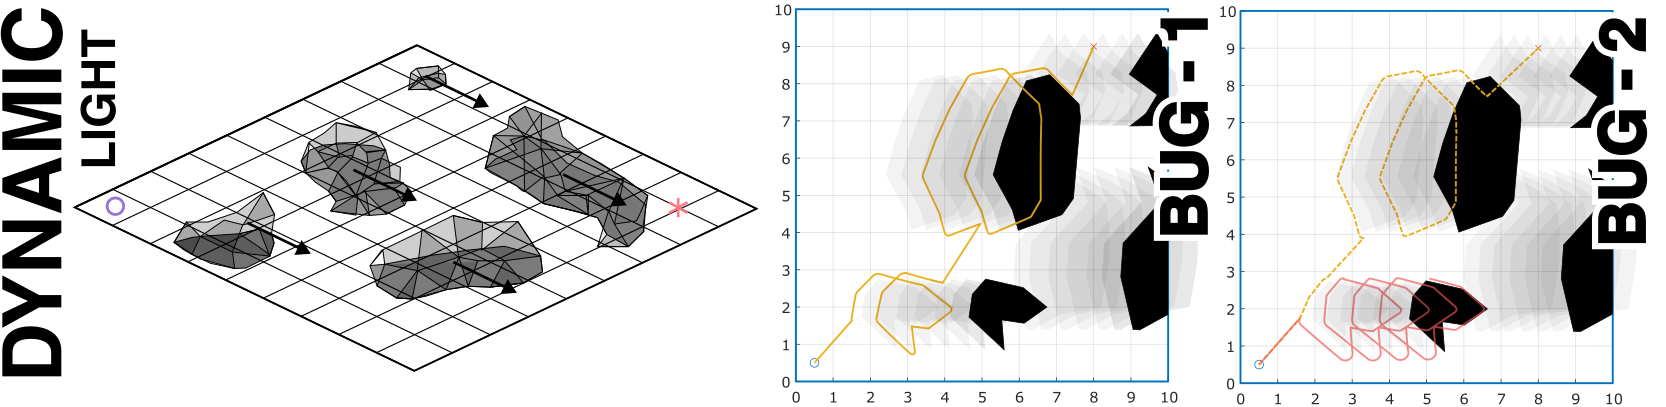
\includegraphics[width=1.0\linewidth]{figures/DYNAMIC-1.pdf}
     \end{center}
     % \vspace{-1em}
     \caption{Dynamic scenario, obstacles are moving to the right at a steady rate. Bug-2 was faster to reach the goal but somewhat unreliable.}
     \label{dynamic-1}
     %\vspace{-1em}
\end{figure*}

\begin{figure*}[t!]
    \begin{center}
        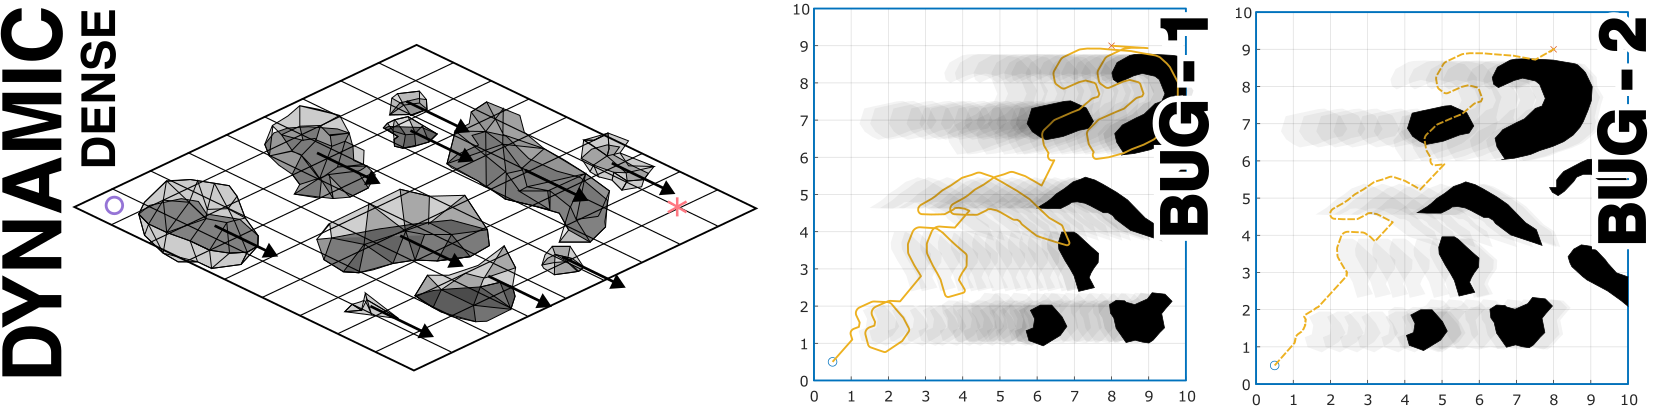
\includegraphics[width=1.0\linewidth]{figures/DYNAMIC-2.pdf}
     \end{center}
     %\vspace{-1em}
     \caption{Dynamic scenario with dense environment, Bug-2 outperforms Bug-1.}
     \label{dynamic-2}
     \vspace{-1em}
\end{figure*}

\subsection{\fontsize{10}{13}\selectfont DYNAMIC}

In a dynamic environment, the asteroids, which in our context are represented by planar polygons, exhibit non-negligible motion with respect to the space probe's position. This dynamic element introduces a level of complexity into the navigation process, as the obstacles are no longer static but can potentially collide with the probe's path. The dynamic environment prepared is a simple one, all the obstacles have the same speed and move in the same direction hence the relative distances are the same. This simplification also handles the situations on which the obstacles came to collide.

The Bug1's take on the dynamic obstacles is time consuming, circumnavigating a large obstacle takes some time and the obstacle is moving that means the total displacement is larger and hence the bug might unintentionally get further away from the goal. Another comment on the situation is that, the closest point on the obstacle can change when in movement.

The Bug2's shot on dynamic obstacles is more greedy, this can be observed on Fig.~(\ref{dynamic-1}), where Bug2 exists the obstacle as it passes through the m-line however the obstacles movement causes it to consider the same obstacle as a new one and begins another round of going through it. If this phoneme happening again and again, it can cause the bug to drift to away with the obstacle and puts in a situation where it might never cross the m-line again. In this situation the bug is deemed to circumnavigate the obstacle indefinitely.

\begin{figure*}[b!]
    \begin{center}
        \includegraphics[width=1.0\linewidth]{figures/COMP-TABLE.png}
     \end{center}
     \vspace{-1em}
     \caption{Computation time comparison for all the cases.}
     % renkleri üstteki figüre göre yapabiliriz
     \label{comp-table}
     \vspace{-1em}
\end{figure*}


\section{\large \textbf{Observations}}

The trend in observations of these scenarios came to show that the very nature of the algorithms, this being the more cautious planning of Bug-1 and the greediness of the Bug-2 also seen in dynamic scenarios. To delve more on the examples, in comparison of static and dynamic cases Bug-1 is more aware of obstacle being an obstacle and leaves it once it encounters the closest point, the closest point is still a point on the obstacle hence for the situations where the obstacle is moving through the goal the bug will still leave the obstacle. However Bug-2 checks the m-line to leave the obstacle but in dynamic scenarios this approach is very tricky since it would require a new definition on m-line. An approach on that would consider the keeping track of whether the bug is circumnavigated the obstacle, if yes then a new m-line can be defined on the first point of contact relative to the obstacle. 

Time comparisons have been conducted across various experimental scenarios. The findings reveal that Bug-1 exhibits a worse performance. However, as the dynamic environments become more cluttered the ratio on timing does not change, that means the impact of density of the environment change linearly over time for both algorithms.


\section{\large \textbf{Conclusions}}

In conclusion, this paper worked on bug algorithms and tested those for dynamic environments that is inspired by the space-like dynamic conditions. 
The bug algorithms performed in a consistent nature to their individual intends. Also results indicate that there is a gap to be filled on Bug-2 algorithm to exhibit a better convergence of the solution.

For future investigations, there is a clear need for improvements. Upcoming experiments are envisioned to include differentiating the obstacle sizes, changing the direction of the group of obstacles such and the goal location in a sense that the probe is moving upstream or downstream in the flow. A new dimension could be introduced by non-planar entities that are in higher dimensions. Projection of those into planar world would be as shape-changing polygons in which the performance comparison between bugs can change drastically.

\bibliographystyle{bib/IEEEtaes}

\bibliography{bib/refs}\ %IEEEabrv instead of IEEEfull

\end{document}
